\subsection{Модель трехатомного гидрида с двумя колебательными и одной деформационной степенями свободы.}

Рассмотрим модель трехатомного гидрида с одной деформационной и двумя валентными степенями свободы. Предыдущая модель доказала, что основной вклад в колебательно-вращательное взаимодействие вносит именно колебание деформационного типа. Данная модель позволит уточнить полученные результаты, и покажет насколько сильно влияние валентных колебаний на систему, испытывающую колебательно-вращательное движение. \\
В рамках данной модели мы также будем предполагать, что масса центрального атома много больше крайних атомов. На рис.\eqref{fig:triatomic_full} молекула изображена в подвижной системе координат, система координат выбрана так же, как это было сделано в предыдущей модели. Обозначим расстояния между легкими и тяжелым атомами $r_1$ и $r_2$.

\begin{figure}[H]
  \centering
	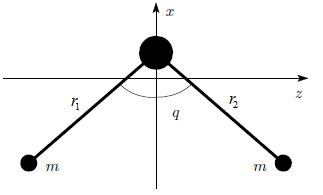
\includegraphics[width=0.4\textwidth]{../pictures/triatomic_full.png}
	\caption{Молекула $\ce{H2X}$ в подвижной системе отсчета.}
	\label{fig:triatomic_full}
\end{figure}

Выпишем координаты легких атомов в системе координат, связанной с центром масс.
\vverh
\begin{gather}
\left\{
\begin{aligned}
x_1 &= - r_1 \cos \lb \frac{q}{2} \rb \\
y_1 &= 0 \\
z_1 &= - r_1 \sin \lb \frac{q}{2} \rb 
\end{aligned}
\right. \quad \quad \quad
\left\{
\begin{aligned}
x_3 &= - r_2 \cos \lb \frac{q}{2} \rb \\
y_3 &= 0 \\
z_3 &= r_2 \sin \lb \frac{q}{2} \rb
\end{aligned}
\right.\notag
\end{gather}

Запишем кинетическую энергию в форме Лагранжа в подвижной системе координат. Используем формулы, приведенные в первой части, определяющие вид матриц $\bba$, $\bbA$, $\bbI$ в общем случае. Количество степеней свободы в данной модели равно $s = 3$, следовательно, размеры всех вышеперечисленных матриц будут равны $\dim \bba = \dim \bbA = \dim \bbI = 3 \times 3$. Путем несложных преобразований приходим к следующему виду матрицы тензора инерции (который в рамках данной модели не является диагональным):
\vverh
\begin{gather}
\bbI = \begin{pmatrix}
m \left( r_1^2 + r_2^2 \right) \sin^2 (\frac{q}{2}) & 0 & m \left( r_2^2 - r_1^2 \right) \sin (\frac{q}{2}) \cos(\frac{q}{2}) \\
0 & m (r_1^2 + r_2^2) & 0 \\
m \left( r_2^2 - r_1^2 \right) \sin(\frac{q}{2}) \cos(\frac{q}{2}) & 0 & m \left( r_1^2 + r_2^2 \right) \cos^2 (\frac{q}{2})
\end{pmatrix} \notag
\end{gather}

Составлять матрицы $\bba$, $\bbA$ будем таким образом, чтобы они давали правильные выражения кинетической энергии (в любом представлении) при использовании вектора обобщенных координат в форме $\begin{bmatrix} r_1 \\ r_2 \\ q \end{bmatrix}$. Матрица $\bba$ оказывается диагональной, причем пара диагональных элементов оказывается равной (в следствие идентичности, с точностью до номера, атомов $1$ и $3$): $a_{11} = a_{22} = m, \, a_{33} = \frac{m}{4} (r_1^2 + r_2^2)$. Матрица $\bbA$, в отличие от прошлой модели, не является нулевой, она содержит единственный ненулевой элемент: $A_{23} = \frac{m}{2} (r_2^2 - r_1^2)$. Заметим, что при фиксировании двух длин связи $r_2 = r_1 = r_0$, матрица $\bbA$ становится нулевой. \\
С учетом выполненных преобразований запишем кинетическую энергию лагранжевого вида в скалярной форме: 
\vverh
\begin{gather}
T_\mathcal{L} = \frac{1}{2} m \left(\dot{r}_1^2 + \dot{r}_2^2 + ( r_1^2 + r_2^2 ) \frac{\dot{q}^2}{4} \right) + \Omega_y m \frac{\dot{q}}{2} (r_2^2 - r_1^2 ) + \frac{1}{2} \vec{\Omega}^{\, \top} \, \bbI \, \vec{\Omega} \notag 
\end{gather}

Для перехода к кинетической энергии в форме Гамильтона применим формулы, полученные при помощи подхода Фробениуса к обращению блочных матриц. Достаточно длинные выкладки приводят к следующему виду элементов блочной матрицы $\bbG$, которая определяет вид кинетической энергии в гамильтоновой форме:
\vverh
\begin{gather}
\bbG_{11} = \frac{r_1^2 + r_2^2}{2 m r_1^2 r_2^2}
\begin{pmatrix}
\frac{1}{1 - \cos q} & 0 & \frac{r_1^2 - r_2^2}{r_1^2 + r_2^2}  \frac{1}{\sin q} \\
0 & 1 & 0 \\
\frac{r_1^2 - r_2^2}{r_1^2 + r_2^2} \frac{1}{\sin q} & 0 & \frac{1}{1 + \cos q}
\end{pmatrix} \notag
\end{gather}